\documentclass[xcolor=dvipsnames]{beamer}
%\documentclass[handout,xcolor=dvipsnames]{beamer}

% == Packages for beamer
\usepackage{xcolor}
\usepackage{graphicx}
\usepackage{fancybox}
\usepackage{hyperref}
\usepackage{amsmath,amssymb,amsfonts,bm}
\usepackage{wasysym}
\usepackage{colortbl}
\usepackage{booktabs}
\usepackage[english]{babel}
\usepackage{times}
\usepackage[T1]{fontenc}

% == Other Packages
\usepackage{rotating}
\usepackage{latexsym}
\usepackage{ulem}
\usepackage{appendixnumberbeamer}

% == theme & colors
\usetheme{Warsaw}
\usepackage{helvet}
\definecolor{someblue}{rgb}{0,.1,0.8}
\definecolor{dgreen}{rgb}{0,.6,0.8}
\useoutertheme{infolines}

% == New Commands
\newcommand\spacingset[1]{\renewcommand{\baselinestretch}{#1}\small\normalsize}
\renewcommand\r{\right}
\renewcommand\l{\left}
\newcommand\makegaps{\addtolength{\itemsep}{.25\baselineskip}}
\newcommand\makebiggaps{\addtolength{\itemsep}{.5\baselineskip}}

% = For stats & econometrics
\renewcommand{\epsilon}{\varepsilon}
\newcommand\ud{\mathrm{d}}
\newcommand\dist{\buildrel\rm d\over\sim}
\newcommand\ind{\stackrel{\rm indep.}{\sim}}
\newcommand\iid{\stackrel{\rm i.i.d.}{\sim}}
\newcommand\logit{{\rm logit}}
\newcommand\cA{\mathcal{A}}
\newcommand\cN{\mathcal{N}}
\newcommand\E{\mathbb{E}}
\newcommand\V{\mathbb{V}}
\newcommand\cJ{\mathcal{J}}
\newcommand\y{{\bm y}}
\newcommand\Y{{\bm Y}}
\newcommand\X{{\bm X}}
\newcommand\x{{\bm x}}
\newcommand\eps{{\bm\varepsilon}}
\newcommand\zero{{\bm 0}}
\newcommand\be{{\bm\beta}}
\renewcommand\b{{\bm b}}
\newcommand\C{{\bm C}}
\newcommand\D{{\bm D}}
\newcommand\I{{\bm I}}
\newcommand\Z{{\bm Z}}
\newcommand\eeta{{\bm \eta}}
\newcommand{\Var}{\mathrm{Var}}
\newcommand{\Cov}{\mathrm{Cov}}

\DeclareMathOperator*\plim{plim}
\DeclareMathOperator\rank{rank}
\newcommand\indep{\protect\mathpalette{\protect\independenT}{\perp}}
\DeclareMathOperator{\sgn}{sgn}
\def\independenT#1#2{\mathrel{\rlap{$#1#2$}\mkern2mu{#1#2}}}

\newtheorem{assumption}{Assumption}
\newtheorem{iass}{Identification Assumption}
\newtheorem{ires}{Identification Result}
\newtheorem{estm}{Estimand}
\newtheorem{esti}{Estimator}

\newcommand{\notindep}{{\bot\negthickspace\negthickspace\bot}{\negthinspace
  \negmedspace \negthickspace \negthickspace \diagup
  \;}}
\newcommand{\bs}{\boldsymbol}
\newcommand{\mb}{\mathbf}
\newcommand{\real}{\mathbb{R}}
\renewcommand{\u}{\ensuremath{\mb{u}}}
\renewcommand{\v}{\ensuremath{\mb{v}}}
\newcommand{\U}{\ensuremath{\mb{U}}}
\newcommand{\M}{\ensuremath{\mb{M}}}
\renewcommand{\b}{\ensuremath{\bs{\beta}}}
\newcommand{\e}{\ensuremath{\bs{\epsilon}}}
\newcommand{\bhat}{\ensuremath{\hat{\bs{\beta}}}}
\newcommand{\XX}{\ensuremath{\X'\X}}
\newcommand{\XXinv}{\ensuremath{\left(\XX\right)^{-1}}}
\newcommand{\hatsig}{\ensuremath{\hat{\sigma}^2}}
\newcommand{\sig}{\ensuremath{\sigma^2}}
\newcommand{\hatmat}{\ensuremath{\X \XXinv \X'}}
\newcommand{\ehat}{\ensuremath{\hat{\e}}}
\newcommand{\tr}{\text{tr}}
\newcommand{\Sig}{\ensuremath{\bs{\Sigma}}}
\newcommand{\SigInv}{\ensuremath{\bs{\Sigma^{-1}}}}
\newcommand{\W}{\ensuremath{\mb{W}}}

\graphicspath{{images/}}

\title[]{Experiments}
\subtitle[ ]{Stat 256, Causality}
\date{Spring 2026}
\author[Hazlett]{Chad Hazlett }
\institute[UCLA]{UCLA\\[1ex]
  \texttt{chazlett@ucla.edu}
}


\begin{document}

\begin{frame}
  \titlepage
\end{frame}


%% =====================================================================
\section{Identification}
%% =====================================================================

\begin{frame}
  \frametitle{Identification vs.\ Estimation}
  \small
Goal: learn about an \textit{unobservable, counterfactual-dependent} quantity of interest using \textit{observed} data.\\

\pause
\medskip
Two inferential hurdles:
\begin{enumerate}
\item \alert{Identification}: With data on an entire population, can you recover your QoI?
\item \alert{Estimation}: With finite data on a sample, how well can you learn it?
\end{enumerate}
\pause
\begin{center}
\textbf{Identification precedes estimation.}
\end{center}

\pause
\medskip
For each identification strategy we discuss:
\footnotesize
\begin{enumerate}
\item the \textcolor{Blue}{identification assumption}
\item information from outside the data supporting it
\item testable implications (limited)
\item estimators
\item sensitivity to violations
\end{enumerate}
\end{frame}


%% =====================================================================
\section{From POMs to Experiments}
%% =====================================================================

\begin{frame}
\frametitle{Classical Randomized Experiment}
\small
Setup:
\begin{itemize}
\item Units: $i = 1, \ldots, N$
\item Treatment: $D_i \in \{0,1\}$, randomly assigned
\item Potential outcomes: $Y_{0i}$, $Y_{1i}$
\item Observed outcome: $Y_i = D_i Y_{1i} + (1-D_i) Y_{0i}$ \quad (consistency)
\item $N_1 = \sum_{i=1}^N D_i$, \quad $N_0 = N - N_1$
\end{itemize}

\pause
\medskip
Random assignment can take several forms:
\footnotesize
\begin{itemize}
\makegaps
\item \alert{Complete randomization}: Exactly $N_1$ units treated (draw without replacement)
\item \alert{Simple (Bernoulli) randomization}: Each unit independently assigned with $\Pr(D_i=1)=p$
\end{itemize}
\end{frame}


\begin{frame}
  \frametitle{Randomization $=$ Ignorability}
  \small
Random assignment of $D_i$ guarantees:
$$ \l\{ Y_{1i}, \ Y_{0i}\r\} \ \indep \ D_i $$

\pause
\medskip
That is: the potential outcomes a unit \textit{would have} under treatment or control are statistically independent of which group they are assigned to.\\

\pause
\bigskip
This is the \textcolor{Blue}{identification assumption} for experiments.  Let's see what it buys us.
\end{frame}


\begin{frame}[t]
\frametitle{Identification of ATE Under Experiments}
\small
\onslide<1-> \textcolor{Blue}{Quantity of Interest}:
$$ \tau_{ATE} \ \equiv \ \E[Y_{1i} - Y_{0i}]$$

\onslide<2-> \textcolor{Blue}{Identification}:\quad Using $(Y_{1i},Y_{0i}) \indep D_i$,\\
\footnotesize
\onslide<3-> \begin{eqnarray*}
\E[Y_{1i}] - \E[Y_{0i}] &=& \E[Y_{1i}|D_i=1] - \E[Y_{0i} | D_i=0] \quad (\text{by ignorability}) \\
&=& \E[Y_{i}|D_i=1] - \E[Y_{i} | D_i=0]  \quad (\text{by consistency})\\
&=& \text{DIM estimand}
\end{eqnarray*}
\onslide<4-> \small Practice these two steps.  They are the core of every ID argument we will see.
\end{frame}


\begin{frame}
\frametitle{Identification of Full Distributions}
\small
With $(Y_1,Y_0) \indep D$, we identify more than means.

\begin{ires}\small
Let $F_{Y_d}(y)$ denote the CDF of $Y_d$.  Then
\begin{eqnarray*}
F_{Y_0}(y) &=& \Pr(Y_0\leq y) = \Pr(Y_0\leq y \mid D=0) = \Pr(Y\leq y \mid D=0) \\
F_{Y_1}(y) &=& \Pr(Y\leq y \mid D=1)
\end{eqnarray*}
So the effect at any quantile $\theta\in[0,1]$ is identified:
\[
\alpha_{\theta}=Q_\theta(Y_1)-Q_\theta(Y_0)=Q_\theta(Y\mid D\!=\!1)-Q_\theta(Y\mid D\!=\!0)
\]
\end{ires}

\pause
\medskip
Note: the \textit{quantile of the effect} $Q_\theta(Y_1 - Y_0)$ is \textbf{not} identified without further assumptions --- the difference of quantiles is not the quantile of the difference.
\end{frame}


%% =====================================================================
\section{Estimation and Inference}
%% =====================================================================

\begin{frame}{SATE and PATE}
\small
\begin{itemize}
\item<1-> \textbf{SATE}: $\tau_{SATE} = \frac{1}{N}\sum_{i=1}^N (Y_{1i} - Y_{0i})$ \medskip
  \begin{itemize}
  \footnotesize
   \item Inferences limited to units in the study
   \item Resampling notion can vary:
   \begin{itemize}
   \scriptsize
   \item \textit{Design-based}: $\X$, POs fixed; only treatment assignment is re-randomized
   \item \textit{Model-based}: $\X$, $D$ fixed; residual influences on $Y$ are random
   \end{itemize}
  \end{itemize}\bigskip
\item<2-> \textbf{PATE}: $\tau_{PATE} = \E[Y_{1i} - Y_{0i}]$ over a superpopulation \medskip
 \begin{itemize}
  \footnotesize
  \item Generalizes the above to also redraw units from a larger superpopulation/DGP
  \end{itemize}\bigskip
\item<3-> If sampling is random from the population, $\E[\text{SATE}]=\text{PATE}$.  We are often uninterested in distinguishing them.
\end{itemize}
\end{frame}


\begin{frame}{Variance of the DIM: PATE}
\small
\onslide<1-> Start from the variance of the mean difference:
\[
\V(\hat\tau) \;=\; \V(\bar Y_1) + \V(\bar Y_0) - 2\Cov(\bar Y_1, \bar Y_0)
\]

\onslide<2-> \textcolor{Blue}{For the PATE} (superpopulation view): treated and control units are independent draws, so $\Cov(\bar Y_1, \bar Y_0) = 0$:
\[
\V_{\text{Neyman}}(\hat\tau) = \frac{\sigma^2_{Y_1}}{N_1} + \frac{\sigma^2_{Y_0}}{N_0}
\]
This is the \textbf{Neyman variance}.\\

\medskip
\onslide<3-> \textcolor{Blue}{Plug-in estimator}: replace population variances with sample variances:
\[
\widehat{SE}(\hat\tau) = \sqrt{\frac{S_1^2}{N_1} + \frac{S_0^2}{N_0}}, \qquad S_d^2 = \frac{1}{N_d-1}\sum_{i:D_i=d}(Y_i - \bar Y_d)^2
\]
\end{frame}


\begin{frame}{Variance of the DIM: SATE}
\small
\onslide<1-> \textcolor{Blue}{For the SATE} (finite-population / design-based view): the potential outcomes $(Y_{1i}, Y_{0i})$ are fixed.  Randomness comes only from treatment assignment.\\

\medskip
\onslide<2-> Under complete randomization, the $N_1$ treated units are a sample \textit{without replacement} from the $N$ fixed units.  Two consequences:
\begin{itemize}
\footnotesize
\item $\V(\bar Y_d)$ is \textit{smaller} than $\sigma^2_{Y_d}/N_d$ by a finite population correction factor $(1 - N_d/N)$
\item $\Cov(\bar Y_1, \bar Y_0) \neq 0$ because the two groups are complementary (selecting one determines the other)
\end{itemize}

\medskip
\onslide<3-> Working through the finite-population sampling algebra, these combine to give:
\[
\V_{SATE}(\hat\tau) = \frac{\sigma^2_{Y_1}}{N_1} + \frac{\sigma^2_{Y_0}}{N_0} - \frac{\sigma^2_\tau}{N}
\]
where $\sigma^2_\tau = \Var(\tau_i) \geq 0$.\\

\medskip
\onslide<4-> So the Neyman variance is \textbf{conservative} for the SATE.  The gap is $\sigma^2_\tau/N$: zero if effects are constant, and shrinking with $N$ regardless.
\end{frame}


\begin{frame}
  \frametitle{Regression to Estimate ATE}
\small
\begin{esti}[Regression with Experiments]\small
\begin{align*}
 Y_i &= D_i Y_{1i} + (1-D_i) Y_{0i} \\
 &= Y_{0i} + (Y_{1i}- Y_{0i}) D_i \\
 &= \underbrace{\bar Y_0}_{\alpha} + \underbrace{(\bar Y_1 - \bar Y_0)}_{\hat\tau} D_i + \underbrace{\{(Y_{0i} - \bar Y_0) + D_i [(Y_{1i} - \bar Y_1) - (Y_{0i} - \bar Y_0)] \}}_{\epsilon_i}
\end{align*}
\end{esti}
\vspace{-.1in}
\begin{itemize}
\footnotesize
\item<2-> This does \textbf{not} assume constant effects: $\hat\tau$ averages over heterogeneous $\tau_i$.
\item<3-> The residual $\epsilon_i$ has different variances under $D=1$ and $D=0$ $\Rightarrow$ heteroskedasticity.
\item<4-> We need a heteroskedasticity-robust SE.
\end{itemize}
\end{frame}


\begin{frame}{The Sandwich Variance Estimator}
\small
\onslide<1-> For OLS with $\hat\beta = (\X'\X)^{-1}\X'\Y$:
\begin{align*}
\widehat\V(\hat\beta \mid \X) &= (\X'\X)^{-1}\X'\;\widehat{\Var(Y\mid \X)}\;\X(\X'\X)^{-1}\\
\onslide<2-> &= (\X'\X)^{-1}\X'\hat\Omega\X(\X'\X)^{-1}
\end{align*}
\onslide<2-> where $\hat\Omega = \text{diag}(\hat\omega_1,\ldots,\hat\omega_N)$ estimates the conditional variance of each $Y_i$.\\[4pt]

\onslide<3-> The choice of $\hat\omega_i$ defines the variant:\\ [4pt]
\footnotesize
\begin{tabular}{@{} l l @{}}
\textbf{HC0}: & $\hat\omega_i = \hat\epsilon_i^2$ \\[2pt]
\textbf{HC1}: & $\hat\omega_i = \frac{N}{N-p}\,\hat\epsilon_i^2$ \quad (global degrees-of-freedom correction)\\[2pt]
\textbf{HC2}: & $\hat\omega_i = \frac{\hat\epsilon_i^2}{1-h_{ii}}$ \quad (leverage correction, $h_{ii}$ = $i$th diagonal of $\X(\X'\X)^{-1}\X'$)
\end{tabular}\\[6pt]
\small

\onslide<4-> With HC0, the ``meat'' of the sandwich becomes:
\[
\X'\hat\Omega\X = \sum_{i=1}^N \hat\epsilon_i^2\, \x_i \x_i'
\]
where $\hat\epsilon_i = Y_i - \x_i'\hat\beta$ and $\x_i$ is the $i$th row of $\X$.
\end{frame}


\begin{frame}{Sandwich for the Experimental Regression}
\small
\onslide<1-> The $[2,2]$ element of $(\X'\X)^{-1}\X' \text{diag}(\hat{\epsilon}_i^2) \X(\X'\X)^{-1}$ is just 
\[\widehat{\V}(\hat{\tau}) = (\tilde{D}'\tilde{D})^{-1}\tilde{D}' \text{diag}(\hat{\epsilon}_i^2) \tilde{D}(\tilde{D}'\tilde{D})^{-1}\]
where $\tilde{D}$ is the vector $D_i - \bar D$. This sorts and splits into two pieces:\\
\scriptsize
\[
= \frac{\displaystyle\sum_{i:\,D_i=1} \hat\epsilon_i^2\, \tilde D_i^2}{\left(\tilde D'\tilde D\right)^2} + \frac{\displaystyle\sum_{i:\,D_i=0} \hat\epsilon_i^2\, \tilde D_i^2}{\left(\tilde D'\tilde D\right)^2}
\]

\onslide<2-> \footnotesize Noting that $\tilde D_i = N_0/N$ for treated, and $-N_1/N$ for controls, and that $\tilde D'\tilde D = N_1 N_0/N$, after some tedious algebra we get this to equal

\scriptsize
\[
= \frac{\widehat{\Var}(Y|D=1)}{N_1} + \frac{\widehat{\Var}(Y|D=0)}{N_0}
\]
\onslide<3-> \footnotesize Further, if you construct $\widehat{\Var}(Y|D\!=\!d)$ with the $N_d-1$ correction then you have the HC2 correction and this matches Neyman exactly.

%\footnotesize
%
%\[
%= \frac{N_1 \tilde S_1^2 \cdot (N_0/N)^2}{(N_1 N_0/N)^2} + \frac{N_0 \tilde S_0^2 \cdot (N_1/N)^2}{(N_1 N_0/N)^2} \;=\; \frac{\tilde S_1^2}{N_1} + \frac{\tilde S_0^2}{N_0}
%\]
%\small where $\tilde S_d^2 = \frac{1}{N_d}\sum_{i:D_i=d}(Y_i - \bar Y_d)^2$.\\
%
%\medskip
%\onslide<5-> \textbf{HC2 matches Neyman exactly.}  Here $h_{ii} = 1/N_{D_i}$, so dividing $\hat\epsilon_i^2$ by $(1-h_{ii})$ replaces each $N_d$ with $N_d\!-\!1$:
%\[
%\widehat\V_{HC2}(\hat\tau) = \frac{S_1^2}{N_1} + \frac{S_0^2}{N_0} = \widehat\V_{\text{Neyman}}(\hat\tau)
%\]
\end{frame}


\begin{frame}
  \frametitle{Example: Effect of Job Training on Earnings}
\small
\begin{itemize}
  \item Treatment: $N_1=7{,}487$, \quad $\bar{Y}_1 = \$16{,}199$, \quad $S_1 = \$17{,}038$
  \item Control: $N_0=3{,}717$, \quad $\bar{Y}_0 = \$15{,}040$, \quad $S_0 = \$16{,}180$
  \medskip
  \item<2-> $\hat\tau = 16{,}199 - 15{,}040 = \$1{,}159$ \medskip
  \item<3-> $\widehat{SE} = \sqrt{\dfrac{17{,}038^2}{7{,}487}+ \dfrac{16{,}180^2}{3{,}717}} \approx \$330$
  \medskip
  \item<4-> $t = 1{,}159\,/\,330 \approx 3.5$, \quad $p \approx 0.0005$
\end{itemize}
\bigskip
\onslide<5-> \footnotesize All exactly the same thing:
\begin{itemize}
 \item DIM with Neyman SE
 \item Welch (unequal variance) $t$-test
 \item  \texttt{lm(earnings $\sim$ D)} with HC2 SEs via \texttt{sandwich::vcovHC(fit, type="HC2")}
 \end{itemize}
\end{frame}


%% =====================================================================
\section{Randomization Inference}
%% =====================================================================

\begin{frame}\frametitle{Fisher's Exact Test}
\small
\onslide<1-> You already know the large-$N$ test:
\[
H_0:\E[Y_1] =\E[Y_0],\quad H_1:\E[Y_1] \neq\E[Y_0]  \qquad \text{(weak null)}
\]
\pause

Fisher's Exact Test uses a stronger hypothesis:
\[
H_0: Y_{1i} = Y_{0i} \;\; \forall\, i  \qquad \text{(sharp null of no effect)}
\]

\pause
\medskip
\alert{Key idea}: Under the sharp null, we ``observe'' all potential outcomes --- so we can compute the test statistic under every possible treatment assignment.\\

\pause
\medskip
Procedure:
\footnotesize
\begin{enumerate}
\item Compute $\hat\tau_{\text{obs}}$ from actual assignment
\item For every (or many) alternative assignments $\omega \in \Omega$, compute $\hat\tau(\omega)$ using the filled-in PO schedule
\item $p$-value $= \Pr_\omega\!\bigl(|\hat\tau(\omega)| \geq |\hat\tau_{\text{obs}}|\bigr)$
\end{enumerate}
\end{frame}


% -- Fisher small-sample example: expanding table --
\begin{frame}
\frametitle{Fisher's Exact Test: Small-Sample Example}
\small
\only<1>{%
\begin{center}
\begin{tabular}{@{} c c c c @{}}
\toprule
$i$ & $Y_{1i}$ & $Y_{0i}$ & $D_i$ \\
\midrule
\rowcolor{blue!8}  1 & 3 & \textcolor{red!70!black}{?} & 1 \\
\rowcolor{blue!8}  2 & 1 & \textcolor{red!70!black}{?} & 1 \\
                    3 & \textcolor{red!70!black}{?} & 0 & 0 \\
                    4 & \textcolor{red!70!black}{?} & 1 & 0 \\
\midrule
$\hat\tau_{\text{obs}}$ & & & 1.5 \\
\bottomrule
\end{tabular}
\end{center}
\bigskip
What do we know given $H_0: Y_{1i} = Y_{0i}\;\;\forall\,i$?
}

\only<2>{%
\begin{center}
\begin{tabular}{@{} c c c c @{}}
\toprule
$i$ & $Y_{1i}$ & $Y_{0i}$ & $D_i$ \\
\midrule
\rowcolor{blue!8}  1 & 3 & \textcolor{red!70!black}{3} & 1 \\
\rowcolor{blue!8}  2 & 1 & \textcolor{red!70!black}{1} & 1 \\
                    3 & \textcolor{red!70!black}{0} & 0 & 0 \\
                    4 & \textcolor{red!70!black}{1} & 1 & 0 \\
\midrule
$\hat\tau_{\text{obs}}$ & & & 1.5 \\
\bottomrule
\end{tabular}
\end{center}
\bigskip
Sharp null fills in the full schedule.  Now enumerate $\binom{4}{2}=6$ assignments.
}

\only<3>{%
\begin{center}
\begin{tabular}{@{} c c c c !{\color{gray!50}\vrule} c c c c c @{}}
\toprule
$i$ & $Y_{1i}$ & $Y_{0i}$ & $D_i$ & $\omega_1$ & $\omega_2$ & $\omega_3$ & $\omega_4$ & $\omega_5$ \\
\midrule
  1 & 3 & \textcolor{red!70!black}{3} & 1 & 1 & 1 & 0 & 0 & 0 \\
  2 & 1 & \textcolor{red!70!black}{1} & 1 & 0 & 0 & 1 & 1 & 0 \\
  3 & \textcolor{red!70!black}{0} & 0 & 0 & 1 & 0 & 1 & 0 & 1 \\
  4 & \textcolor{red!70!black}{1} & 1 & 0 & 0 & 1 & 0 & 1 & 1 \\
\midrule
$\hat\tau(\omega)$ & & & 1.5 & 0.5 & 1.5 & $-1.5$ & $-0.5$ & $-1.5$ \\
\bottomrule
\end{tabular}
\end{center}
\bigskip
$\Pr\!\bigl(|\hat\tau(\omega)| \geq 1.5\bigr) = 4/6 \approx 0.67$. \\[4pt]
Design-based: fixed POs, $D$ varies under re-randomization.  No distributional assumptions.
}
\end{frame}


\begin{frame}{Scaling Up}
\small
With 4 units and 2 treated: $\binom{4}{2}=6$ assignments --- enumerate all.\\
\bigskip
\onslide<2-> With 50 units and 25 treated: $\binom{50}{25} \approx 1.26 \times 10^{14}$.\\
\bigskip
\onslide<3-> Solution: \alert{sample} from $\Omega$.
\begin{itemize}
\item Re-draw treatment assignment many times (e.g.\ 10,000)
\item Compute $\hat\tau(\omega)$ each time under the sharp null
\item Compare observed $\hat\tau$ to this simulated null distribution
\end{itemize}
\end{frame}


\begin{frame}{Randomization Inference in Practice}
\vspace{-.3cm}
\begin{center}
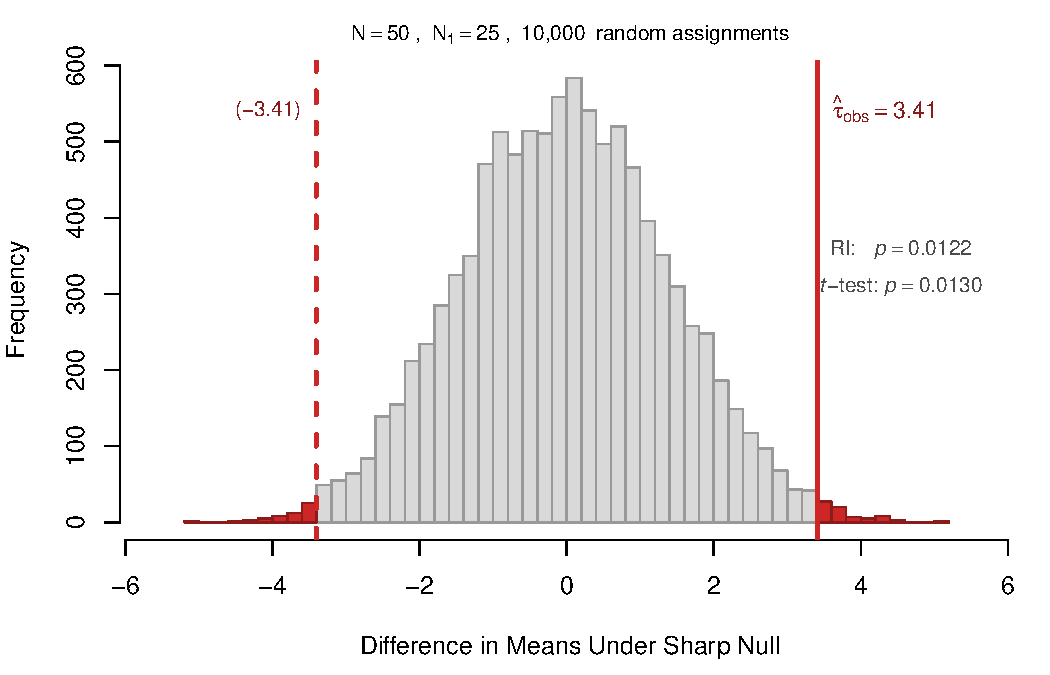
\includegraphics[width=.78\linewidth]{ri_null_distribution.pdf}
\end{center}
\vspace{-.2cm}
\footnotesize
\onslide<2-> Histogram: 10,000 re-randomizations under the sharp null.\\
Solid line: observed $\hat\tau$.  Shaded: values at least as extreme $\Rightarrow$ p-value.
\end{frame}


\begin{frame}{How Do These Inferences Differ?}
\small
\onslide<1-> \textbf{Finite-sample exactness.}\\
\footnotesize
\begin{itemize}
\item The RI p-value is exact under the sharp null --- no CLT required.
\item When $N$ is large, the null distribution is approximately normal and you get nearly the same answer as the $t$-test.
\end{itemize}

\medskip
\onslide<2-> \small\textbf{Sharp null $\neq$ weak null, but close in practice.}\\
\footnotesize
\begin{itemize}
\item The sharp null says $Y_{1i}=Y_{0i}$ for \textit{every} unit.
\item But a summary statistic like the DIM is only sensitive to effects that \textit{accumulate} --- not to effects that cancel.  Rejecting the sharp null via the DIM really tells you ``effects exist \textit{and} don't average to zero,'' which is close to the weak null.
\end{itemize}

\medskip
\onslide<3-> \small\textbf{RI vs.\ the bootstrap.}\\
\footnotesize
\begin{itemize}
\item (Paired) bootstrap resamples \textit{units} --- ``what if we'd drawn different people?'' (superpopulation).
\item RI re-randomizes \textit{treatment} within the fixed sample --- ``what if the same people got different assignments?'' (design-based).
\end{itemize}

\medskip
\onslide<4-> \small \textbf{Bottom line}: RI most valuable in \alert{small samples} where CLT inference is suspect.
\end{frame}


%% =====================================================================
\section{Clustering}
%% =====================================================================

\begin{frame}{When Observations Are Not Independent}
\small
\onslide<1-> Everything so far assumed (conditionally) independent observations.  Often violated:
\begin{itemize}
\footnotesize
\item Voters in the same precinct
\item Students in the same classroom
\item Repeated measures on the same person
\end{itemize}

\medskip
\onslide<2-> Two distinct problems:\\[4pt]
\begin{enumerate}
\item<2-> \textbf{Clustered assignment.}  Treatment assigned at group level (village, school, precinct).  This inflates the \textit{actual} variance of $\hat\tau$ --- you have less independent information than $N$ suggests.
\medskip
\item<3-> \textbf{Correlated residuals.}  Suppose there are cluster level influences, $U_c$, driving within-group correlation in $\epsilon_i$. When combined with cluster-assignment or non-random assignment allowing $D$ correlated with $U_c$ within clusters, this will make HC SE wrong. 
\end{enumerate}

\end{frame}


\begin{frame}{A DGP for Clustering}
\small
\onslide<1-> Units $i$ belong to clusters $c \in \{1,\ldots,C\}$:
\vspace{-4pt}
\[
Y_i = \tau\, D_i + U_{c(i)} + \varepsilon_i
\]
\vspace{-14pt}
\begin{itemize}
\footnotesize
\item $U_c$ is a \textbf{cluster-level} component (precinct culture, school quality, \ldots)
\item $\varepsilon_i$ is individual-level noise, independent across units
\end{itemize}

\medskip
\onslide<2-> \textbf{Individual-level} randomization: each cluster has both treated and control units.  The within-cluster DIM cancels $U_c$ from the comparison --- both arms share the same $U_c$.

\medskip
\onslide<3-> \textbf{Cluster-randomization}: $D_i = D_{c(i)}$.  Now in any given sample, $U_c$ and $D$ are correlated (the treated clusters happen to have higher or lower $U_c$ than the control clusters), shifting $\hat\tau$ away from $\tau$.  Across samples that shift changes direction, inflating $\Var(\hat\tau)$.

\medskip
\onslide<4-> \textbf{Design effect} quantifies the loss.  With average cluster size $m$ and intra-cluster correlation $\rho$ (fraction of $\Var(Y)$ from $U_c$):
\vspace{-4pt}
\[
\mathrm{DEFF} = 1 + (m-1)\rho, \qquad
N_{\mathrm{eff}} = \frac{N}{\mathrm{DEFF}}.
\]
\vspace{-14pt}

\onslide<5-> \footnotesize Example: $N = 1000$, $m = 20$, $\rho = 0.2 \Rightarrow \mathrm{DEFF} = 1 + 19 \times 0.2 = 4.8$, so $N_{\mathrm{eff}} \approx 208$.
\end{frame}


\begin{frame}{Simulation: Simple DIM}
\small
\onslide<1-> Running example: a voter-turnout experiment with $N = 1000$ voters
across 50 precincts, $\tau = 0.01$.
\begin{center}
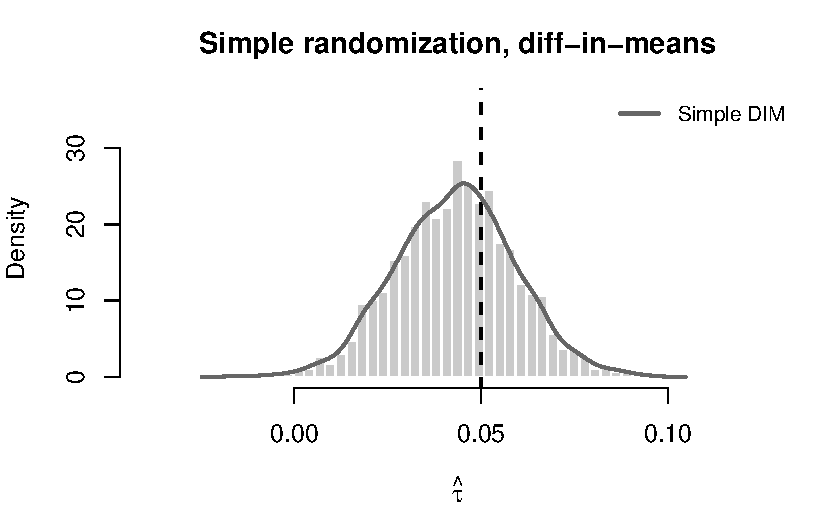
\includegraphics[width=0.65\textwidth]{images/sim_simple.pdf}
\end{center}
\footnotesize
\begin{itemize}
\item<2-> Blue: sampling distribution of $\hat\tau$ under individual-level randomization.
\item<2-> SD(actual) = 0.016; Mean HC2 SE = 0.016. \checkmark
\end{itemize}
\end{frame}


\begin{frame}{Simulation: Cluster-Randomize at the Precinct Level}
\small
\onslide<1-> Same DGP, but now everyone in a precinct gets the same $D$.
\begin{center}
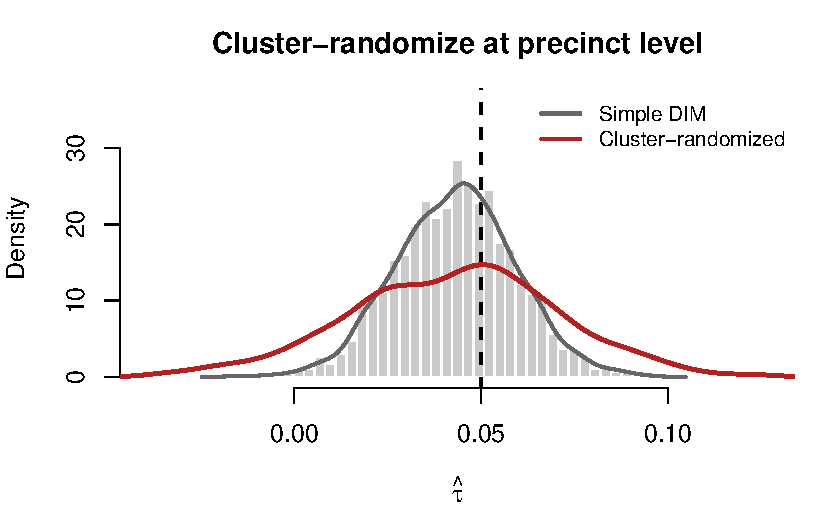
\includegraphics[width=0.65\textwidth]{images/sim_clustered.pdf}
\end{center}
\footnotesize
\onslide<2->
\begin{itemize}
\item Red: sampling distribution under cluster-randomization --- much wider!
\item SD(actual) = 0.028, but Mean HC2 SE = 0.016. \textbf{HC2 is wrong.}
\end{itemize}
\end{frame}


\begin{frame}{The SE Is Wrong --- but CR-SEs Fix It}
\small
\begin{center}
\begin{tabular}{lccc}
\toprule
Design / Estimator & SD(actual) & HC2 SE & CR-SE (precinct) \\
\midrule
Simple DIM                              & 0.016 & 0.016 & 0.016 \\
Cluster-randomized                      & \textbf{0.028} & \textbf{0.016} & \textbf{0.028} \\
\bottomrule
\end{tabular}
\end{center}
\footnotesize
\onslide<2->
\begin{itemize}
\item HC2 assumes independent residuals.  But $U_c$ + cluster-assignment
  means residuals within a cluster are \textbf{identical} in their $U_c$
  component and identical in $D$ --- the worst case for dependence.
\item<3-> Cluster-robust SE (clustered at precinct level) recovers the
  actual sampling variance.  In R:\\
  \texttt{\quad sandwich::vcovCL(fit, cluster = precinct\_id)}
\item<4-> $U_c$ type influences can mess up HC SEs \textbf{without} cluster-assignment if $cov(U_c,D) \neq 0$ within clusters
\begin{itemize}
\footnotesize
\item issue in non-randomized setting (e.g. observational panel data)
\item occurs even if $U_c$ observed, e.g. cluster-level covariates. 
\end{itemize}
\end{itemize}
\end{frame}


\begin{frame}{Cluster-Robust SEs: The Formula}
\small
\onslide<1-> The cluster-robust (``CR'') sandwich estimator:
\[
\widehat\V_{CR}(\hat\beta) = (\X'\X)^{-1}\left(\sum_{c=1}^C \X_c' \hat\epsilon_c\, \hat\epsilon_c' \X_c\right)(\X'\X)^{-1}
\]
where $\X_c$, $\hat\epsilon_c$ are the rows and residuals for cluster $c$.\\

\medskip
\onslide<2-> Allows \textbf{arbitrary} intra-cluster correlation; assumes clusters are independent.\\

\medskip
\onslide<3-> Practical notes:
\begin{itemize}
\footnotesize
\item<3-> Cluster on the source of dependence in your residuals, not on every grouping you can think of.
\item<4-> With few clusters ($C \lesssim 30$--$50$), CR-SEs are downward biased.  Alternatives: wild cluster bootstrap (\texttt{fwildclusterboot} in R), RI at the cluster level, or aggregate to cluster means.
%\item<5-> If there is \textit{no} cluster-level component in $Y$, or if treatment varies within cluster so the component cancels, then HC2 is fine --- CR-SEs buy nothing and widen CIs.
\end{itemize}
\end{frame}


%% =====================================================================
\section{Improving Precision}
%% =====================================================================

\begin{frame}{Unbiased Is Not Enough}
\small
\onslide<1-> Under random assignment, $\hat\tau = \bar Y_1 - \bar Y_0$ is unbiased for the ATE.\\
\medskip
\onslide<2-> But ``unbiased'' is a statement about averages over hypothetical repetitions.  In any \textit{single} experiment, $\hat\tau$ can be far from $\tau$.\\
\medskip
\onslide<3-> What we care about is \textbf{root mean squared error}:
\[
\text{RMSE}(\hat\tau) = \sqrt{\V(\hat\tau) + \text{Bias}^2} = \sqrt{\V(\hat\tau)} \quad \text{(when unbiased)}
\]

\onslide<4-> So the goal is to \textbf{reduce variance}.  Two levers:
\begin{enumerate}
\item \textbf{Design}: blocking (build balance in before randomization)
\item \textbf{Analysis}: covariate adjustment (remove imbalance after the fact)
\end{enumerate}
\medskip
\onslide<5-> Both exploit the same idea: a pre-treatment covariate $X$ that predicts $Y$ can absorb residual variation.
\end{frame}


\begin{frame}{Blocking: Build the Balance In}
\small
\onslide<1-> \textbf{Idea}: pre-stratify on a strong predictor of $Y$, then randomize treatment \textit{within} each stratum (block).\\
\medskip
\begin{itemize}
\footnotesize
\item<2-> Guarantees exact balance on the blocking variable, in your sample --- not just in expectation.
\item<3-> Within-block variation in $Y$ is smaller, so the within-block DIM is sharper.
\item<4-> Randomization still balances unobserved influences, in expectation.
\end{itemize}

\medskip
\onslide<5-> \textbf{Estimator}: within each block $j$, compute $\hat\tau_j$.  Then weight by block size:
\[
\hat\tau_B = \sum_{j=1}^J \frac{N_j}{N}\, \hat\tau_j
\]

\onslide<6-> Equivalently (when treatment probability is the same in every block): OLS with block fixed effects.
\end{frame}


\begin{frame}{Estimation: regression with block dummies}
\small
\onslide<1-> Two regressions for the same data:
\vspace{-4pt}
\begin{align*}
\text{(CR)} \quad Y_i &= \alpha + \tau_{\mathrm{CR}}\, D_i + \textcolor{red}{\varepsilon_i} \\[4pt]
\text{(BR)} \quad Y_i &= \alpha + \tau_{\mathrm{BR}}\, D_i + \sum_{j=2}^J \beta_j B_{j[i]} + \textcolor{blue}{\varepsilon^{*}_i}
\end{align*}
where $B_{j[i]}$ is a dummy for the $j$-th block.

\medskip
\onslide<2-> Under iid sampling, the sampling variances are:
\vspace{-4pt}
\[
\V(\hat\tau_{\mathrm{CR}}) = \frac{\textcolor{red}{\sigma^2_{\varepsilon}}}{\sum_i (D_i - \bar D)^2}, \qquad
\V(\hat\tau_{\mathrm{BR}}) = \frac{\textcolor{blue}{\sigma^2_{\varepsilon^{*}}}}{\sum_i (D_i - \bar D)^2\,(1 - R^2_D)}
\]
where $R^2_D$ is from regressing $D$ on the block dummies.

\medskip
\onslide<3-> \footnotesize When treatment probability is equal in every block, $R^2_D = 0$ and the denominators match.  So we get pure benefit from $\textcolor{blue}{\sigma^2_{\varepsilon^{*}}} < \textcolor{red}{\sigma^2_{\varepsilon}}$ --- the residual variance after block dummies absorb between-block variation in $Y$.

\medskip
\onslide<4-> \footnotesize (DoF cost: $n{-}k{-}1$ vs $n{-}2$ in denominator of $\widehat\sigma^2$.  Negligible unless many, small blocks.)
\end{frame}


\begin{frame}{Simulation: + Blocking}
\small
\onslide<1-> Block on quartiles of a pre-treatment predictor (e.g., \texttt{past\_turnout}).
\begin{center}
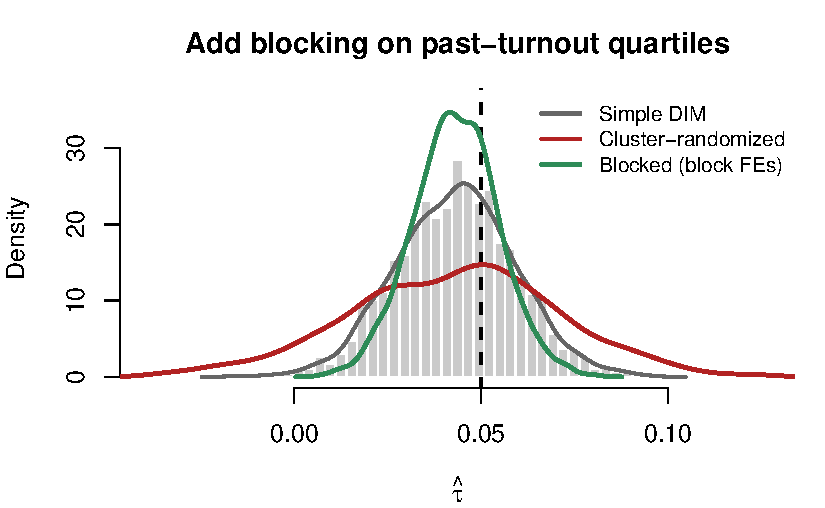
\includegraphics[width=0.65\textwidth]{images/sim_blocked.pdf}
\end{center}
\footnotesize
\begin{itemize}
\item<2-> Green: distribution of $\hat\tau$ under blocking.
\item<2-> SD(actual) = 0.011; tighter than simple DIM (0.016) --- and dramatically tighter than cluster-randomized (0.028).
\item<3-> The gain: blocks balance important $X$ in every sample. 
\end{itemize}
\end{frame}


%\begin{frame}{When Does Blocking Help Most?}
%\small
%\begin{itemize}
%\item<1-> Blocking helps \textbf{a lot} when the blocking variable strongly
%  predicts $Y$.  Within-block variation in $Y$ is small $\Rightarrow$
%  within-block DIM is sharp.
%\medskip
%\item<2-> Blocking on something \textit{unrelated} to $Y$ is free
%  (except a small DoF cost) but useless.
%\medskip
%\item<3-> In our simulation, large gain because
%  $\mathrm{cor}(\text{past\_turnout}, \text{turnout}) \approx 0.8$.
%\medskip
%\item<4-> \textbf{Rule of thumb}: block on the strongest predictor of
%  $Y$ you have.  A pre-treatment version of the outcome is ideal.
%\end{itemize}
%\end{frame}


\begin{frame}{Covariate Adjustment: The Lin Estimator}
\small
\onslide<1-> Consider this regression:
\[
Y_i = \alpha + \tau D_i + \be' X_i + \epsilon_i
\]
\medskip
\onslide<3-> \textbf{Lin (2013)}: demean $X$ and interact with $D$:
\[
Y_i = \alpha + \tau_{Lin} D_i + \be_1'(X_i - \bar X) + \be_2'\, D_i \cdot (X_i - \bar X) + \epsilon_i
\]
\vspace{-.5cm}
\begin{itemize}
\footnotesize
\item<4-> $\tau_{Lin}$ is directly interpretable as the ATE.
\item<4-> Avoids misspecification biases under heterogeneous effects that otherwise lead to ``weird weights'' and Freedman's $O(1/N)$ bias critique.
\item<5-> Use HC2 SEs.  (Pre-specify the covariates if you are worried)
\end{itemize}

\medskip
\onslide<6-> \footnotesize Preview: this is nothing but \textit{regression imputation} / \textit{G-computation} / the \textit{T-learner} --- fit $\hat\mu_d(X)$ separately per arm, impute both POs, average.  We will return to this.\\
\medskip
\onslide<7-> \small \textbf{Best practice}: ``Block on what you can, adjust for what you can't.''
\end{frame}


\begin{frame}{Simulation: all four designs/estimators}
\small
\begin{center}
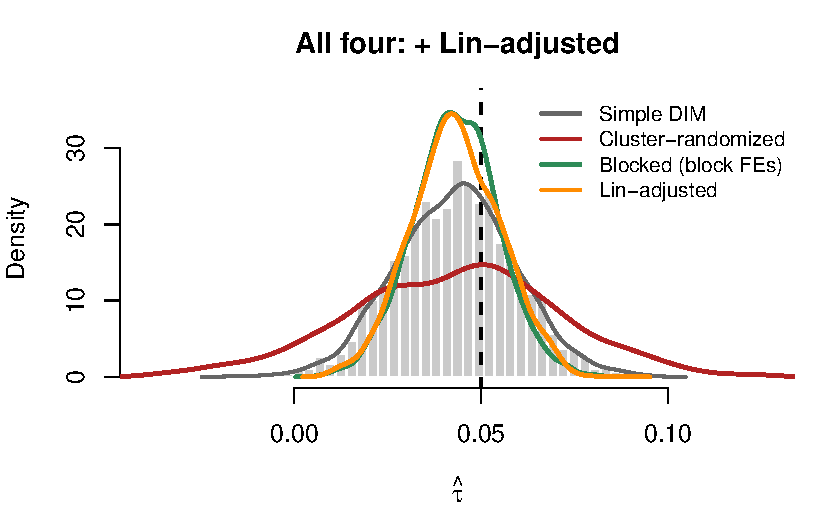
\includegraphics[width=0.72\textwidth]{images/sim_adjusted.pdf}
\end{center}
\footnotesize
\begin{itemize}
\item Orange: Lin-adjusted under individual randomization.
\item<2-> SDs: Simple DIM = 0.016; Cluster = 0.028; Blocked = 0.011; Lin = 0.012.
\item<3-> Blocking and Lin adjustment give similar gains here --- both exploit the same predictor (\texttt{past\_turnout}).
\end{itemize}
\end{frame}


%% =====================================================================
\section{Wrap}
%% =====================================================================

\begin{frame}{Takeaways}
\small
\begin{itemize}
\item \textbf{Randomization $=$ ignorability.}  Identification uses two steps: ignorability, then consistency.
\medskip
\item \textbf{DIM $=$ Neyman $=$ Welch $t$ $=$ OLS with HC2.}
\medskip
\item \textbf{Randomization inference} is exact in finite samples and design-based.  Rejecting the sharp null via DIM is close to rejecting the weak null.
\medskip
\item \textbf{Clustering} inflates variance and/or breaks SE estimation.  Cluster-robust SEs handle it with enough clusters.
\medskip
\item \textbf{Blocking and covariate adjustment} reduce variance --- unbiasedness alone is not the goal.  Block on what you can, adjust for what you can't.
\medskip
\item \textbf{Next}: What if we can't randomize?
\end{itemize}
\end{frame}


%% =====================================================================
\appendix
%% =====================================================================

\begin{frame}
\begin{center}
\Large Appendix
\end{center}
\end{frame}


\begin{frame}
\frametitle{Why Neyman Is Conservative for SATE}
\small
Recall the exact variance:
\[
\V(\hat\tau) = \frac{\sigma^2_{Y_1}}{N_1} + \frac{\sigma^2_{Y_0}}{N_0} - \frac{\sigma^2_{\tau}}{N}
\]

\onslide<2-> The Neyman approximation drops $-\sigma^2_\tau / N$:
\[
\V_{\text{Neyman}}(\hat\tau) = \frac{\sigma^2_{Y_1}}{N_1} + \frac{\sigma^2_{Y_0}}{N_0}
\]

\onslide<3-> Since $\sigma^2_\tau \geq 0$, we have $\V_{\text{Neyman}} \geq \V(\hat\tau)$.\\

\medskip
\onslide<4-> How large is the gap?
\footnotesize
\begin{itemize}
\item If effects are constant ($\tau_i = \tau$ for all $i$), then $\sigma^2_\tau = 0$ and Neyman is exact.
\item If effects vary, Neyman overestimates.  The gap is $\sigma^2_\tau/N$, which shrinks with $N$.
\end{itemize}
\small
\onslide<5-> Either way, CIs based on Neyman SEs have \textit{at least} nominal coverage for the SATE.
\end{frame}


\end{document}
